\documentclass{fwlthesis}
% Add the option final, \documentclass[final]{fwlthesis}, to hide all grey guidance.
% Compile with LuaLaTeX, then BibTeX, then LuaLaTeX twice.

\title{Title of the thesis}
\author{Firstname Lastname}
\studentnumber{s1234567}
\degree{BSc thesis Astronomy}
\supervisors{%
  Supervisor & Prof.~dr.~Name Surname\\
  Daily supervisor & Dr.~Name Surname\\
  Second examiner & Dr.~Name Surname}
\date{Month Year}

\begin{document}
\maketitle

\guidesection{Using this template}
\guide{Grey text like this says what goes where. Write your own text below it. The class option \guidecmd{final} hides all grey text at once, so you can keep it while you write. Compile with LuaLaTeX; in Overleaf, set the compiler to LuaLaTeX in the project settings.}
\guide{\textbf{Citations.} \guidecmd{\textbackslash citet\{key\}} cites in the sentence: \citet{Lichtenberg2021} show that \ldots; \guidecmd{\textbackslash citep\{key\}} cites in parentheses: \ldots{} for millions of years \citep{Lichtenberg2021}. Take the BibTeX entry of each paper from NASA ADS (Export, BibTeX) and keep its key. Cite the journal version once a paper is published, not only the arXiv version. Journal names such as \guidecmd{\textbackslash apj} and \guidecmd{\textbackslash mnras} from ADS work as they are.}
\guide{\textbf{Code and data.} All code and data of the thesis must be public. Put the code, the data and one plotting script per figure in a GitHub repository, make a release, and archive it on Zenodo, which gives it a DOI. Every figure must be replottable from these files: name its data and script in the caption with \guidecmd{\textbackslash figuredata\{link\}}, as in Figure~\ref{fig:cooling}, which \guidecmd{scripts/plot\_cooling.py} plots from \guidecmd{data/cooling.csv}. Cite the codes and data sets of others that you use, in the form their documentation asks for.}
\guide{\textbf{Figures and units.} Plot with the lab style fwl-mpl, save figures as vector PDF, label every axis with its quantity and unit, and use the colours of the style, which stay apart for readers with colour-vision deficiency. A caption starts with what the figure shows and says how to read it: what one line, dot or colour is, and where to look. Write numbers with units as \guidecmd{\textbackslash qty\{1500\}\{\textbackslash kelvin\}}.}
\guide{\textbf{Writing.} Give each paragraph one message, stated in its first sentence. Use the present tense for what the thesis shows and the past tense for what you did. Define every symbol where it first appears. Agree on the plan and the length of each section with your supervisor before you write.}

\section*{Abstract}
\guide{150 to 250 words in 5 labelled parts. Write it last.}
\textbf{Context.} \guide{The problem and why it matters.}
\textbf{Aims.} \guide{The question this thesis answers.}
\textbf{Methods.} \guide{The data, models and codes you used.}
\textbf{Results.} \guide{The main results, as numbers with uncertainties.}
\textbf{Conclusions.} \guide{What follows from the results.}

\section*{Samenvatting}
\guide{The abstract in Dutch, with the same 5 parts.}

\tableofcontents

\section{Introduction}
\label{sec:introduction}
\guide{Start with the scientific context and the open question, with citations to the key papers. Narrow down to the problem of this thesis, state its aim in 1 or 2 sentences, and end with an outline of the next sections.}

\section{Methods}
\label{sec:methods}
\guide{Describe the models, data and codes in enough detail that a reader can reproduce the results: equations with every symbol and unit defined, parameter values (a table helps), and the version of each code. Cite every code and data set you use.}
Following \citet{Lichtenberg2021}, the surface radiates
\begin{equation}
F = \varepsilon\,\sigma T_\mathrm{s}^4 ,
\label{eq:flux}
\end{equation}
with $\varepsilon$ the emissivity, $\sigma$ the Stefan--Boltzmann constant and $T_\mathrm{s}$ the surface temperature, here $T_\mathrm{s} = \qty{1500}{\kelvin}$ at the start.

\section{Results}
\label{sec:results}
\guide{Present the results in the order of your aims, before you interpret them. Refer to every figure in the text. Give numbers with uncertainties and units.}
Figure~\ref{fig:cooling} shows the surface temperature of 3 cases.
\begin{figure}[ht]
  \centering
  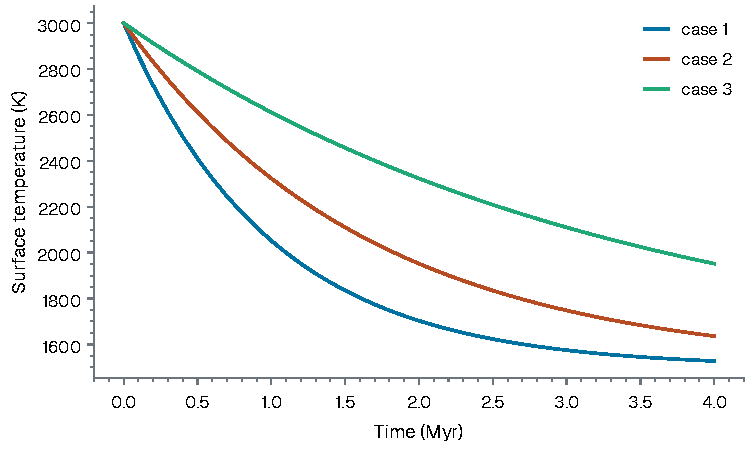
\includegraphics[width=0.75\textwidth]{figures/cooling.pdf}
  \caption{Surface temperature against time for 3 example cases. Each line is one model run.%
    \figuredata{https://doi.org/10.5281/zenodo.0000000}}
  \label{fig:cooling}
\end{figure}

\section{Discussion}
\label{sec:discussion}
\guide{Interpret the results: what they mean, how they compare with earlier work, which assumptions and limits matter most, and what the next step would be.}

\section{Conclusions}
\label{sec:conclusions}
\guide{The main findings, each in 1 or 2 sentences, so that a reader of this section alone knows what the thesis shows.}

\section*{Data and code availability}
\guide{Required. Give the GitHub repository with the release you used and the Zenodo record with its DOI, and say which script makes which figure.}

\section*{Acknowledgments}
\guide{Thank your supervisors and the people who helped. Name the computing facilities and any funding.}

\bibliography{references}

% \appendix
% \section{Appendix title}

\end{document}
